\documentclass[12pt]{article}
\usepackage{fancyhdr}
\pagestyle{fancy}
\fancyhf{}
\fancyfoot[C]{\thepage}
\fancyfoot[L]{\scriptsize CC BY-NC-SA 4.0 \textbullet\ Leo Liang}
\renewcommand{\headrulewidth}{0pt}
\usepackage[margin=1in]{geometry}
\usepackage{amsmath, amssymb}
\usepackage{array, booktabs}
\usepackage{pgffor}
\usepackage{tikz}
\newcommand{\gridaxes}[1]{%
  \draw[step=1,gray!25,very thin] (-#1,-#1) grid (#1,#1);%
  \draw[thick,->] (-#1-0.4,0)--(#1+0.4,0) node[right]{$x$};%
  \draw[thick,->] (0,-#1-0.4)--(0,#1+0.4) node[above]{$y$};%
  \foreach \n in {-#1,...,#1}{\ifnum\n=0\else
      \draw (\n,0.08)--(\n,-0.08) node[below]{\scriptsize$\n$};
      \draw (0.08,\n)--(-0.08,\n) node[left]{\scriptsize$\n$};\fi}%
}
\parindent=0pt
\parskip=1em
\newcolumntype{C}[1]{>{\centering\arraybackslash}p{#1}}
\newcommand{\wl}{\par\vspace{5mm}\noindent\rule{\linewidth}{0.4pt}\par\vspace{1mm}}
\newcommand{\wls}[1]{\foreach \i in {1,...,#1}{\wl}}
% ─────────────────────────────────────────────────────────────────────────────
\begin{document}
\pagestyle{fancy}
\begin{center}
  {\Large\bfseries Final Exam}\\[4pt]
  \vspace{1em}
  Name:\;\underline{\hspace{6cm}}\qquad Time: 2 hours
\end{center}
% =============================================================================
\section*{Instructions}
Use a \textbf{pencil}. \textbf{Show all your work and explain your reasoning} --- you are a mathematician, so a bare answer with no justification will not earn points. Partial credit will be given, so explain your thought process as much as possible, even if you can't answer it. When a question asks you to \textit{explain in words}, write in full sentences. The test is worth 221 points. You have $2$ hours; manage your time, and do not get stuck on any one problem. If something is unclear, ask Leo.

% =============================================================================
\section*{Part 1 --- Speaking Math}

\textbf{1.}\quad[6 pts]\quad Classify each of the following as an \textbf{expression}, an \textbf{equation}, or a \textbf{formula}.

\medskip
\textbf{(a)}\quad $4x$ \hfill \underline{\hspace{4cm}}

\medskip
\textbf{(b)}\quad $y = 5x$ (assume no context is given) \hfill \underline{\hspace{4cm}}

\medskip
\textbf{(c)}\quad $\text{Area} = \text{Width} \cdot \text{Height}$ \hfill \underline{\hspace{4cm}}

\medskip
\textbf{(d)}\quad $3x + 1 = 10$ \hfill \underline{\hspace{4cm}}

\medskip
\textbf{(e)}\quad $12$ \hfill \underline{\hspace{4cm}}

\medskip
In one sentence: what makes something a \textbf{formula} rather than an equation?
\wls{2}

\newpage
\bigskip
\textbf{2.}\quad[10 pts]\quad Consider the expression $\;x^2 y + 8x - 4$.

\medskip
\textbf{(a)}\quad How many terms does it have? \hfill Answer:\;\underline{\hspace{2.5cm}}

\medskip
\textbf{(b)}\quad Fill in the table.

\medskip
\renewcommand{\arraystretch}{2.2}
\begin{tabular}{|C{3cm}|C{3cm}|C{3cm}|C{3cm}|}
\hline
Term & Coefficient & Variable(s) & Exponent(s) \\
\hline
$x^2 y$ & & & \\
\hline
$8x$ & & & \\
\hline
$-4$ & & & \\
\hline
\end{tabular}
\renewcommand{\arraystretch}{1}

\medskip
\textbf{(c)}\quad Mark each True or False. If false, \textbf{write the corrected version}.

\medskip
T\,/\,F\quad The coefficient of the $x$-term is $1$.
\wl

T\,/\,F\quad $-4$ is a term.
\wl

T\,/\,F\quad $x^2 y$ and $8x$ are like terms.
\wl

\newpage
\bigskip
\textbf{3.}\quad[6 pts]\quad Speaking math.

\medskip
\textbf{(a)}\quad Read this aloud and write down the complete English sentence you would say: \[\;x(x-3)^2 + 6\]
\wls{3}

\textbf{(b)}\quad Write the algebraic expression for: ``the quantity four $x$ minus two, over the quantity $x$ plus three.''

\newpage
% =============================================================================
\section*{Part 2 --- Sets}

Recall 
\[
\mathbb{Z} = \{\ldots, -2, -1, 0, 1, 2, \ldots\} \quad \text{(the integers)}
\]
\[
\mathbb{N} = \{1, 2, 3, 4, 5, \ldots\} \quad \text{(the natural numbers)}
\]
\[
\mathbb{R} = \{\ldots, -3.24, 0, 1.99, \sqrt{2}, \pi, 10, \ldots\} \quad \text{(the real numbers)}
\]


\medskip
\textbf{4.}\quad[8 pts]\quad Let $S = \{4,\,8,\,12,\,16\}$.

\medskip
\textbf{(a)}\quad Fill in $\in$ or $\notin$:\qquad
$8 \mathrel{\underline{\hspace{0.8cm}}} S$\qquad
$5 \mathrel{\underline{\hspace{0.8cm}}} S$\qquad
$16 \mathrel{\underline{\hspace{0.8cm}}} S$\qquad
$0 \mathrel{\underline{\hspace{0.8cm}}} S$

\medskip
\textbf{(b)}\quad Write $S$ in set-builder notation (you can use words for the condition).
\wl

\textbf{(c)}\quad Write each in roster notation.
\medskip

\hspace{1.5em}(i)\quad $\{x \in \mathbb{Z} \mid -3 \le x \le 1\}$ $= \;\underline{\hspace{5cm}}$

\medskip
\hspace{1.5em}(ii)\quad $\{x \in \mathbb{N} \mid x^2 < 10\}$ $= \;\underline{\hspace{5cm}}$

\bigskip
\textbf{5.}\quad[4 pts]\quad Subsets.

\medskip
\textbf{(a)}\quad List \textbf{all} subsets of $\{p,\,q\}$ Which one is the \textbf{improper} subset?


\newpage
\bigskip
\textbf{6.}\quad[8 pts]\quad Let $U = \{1,2,3,\ldots,10\}$,\quad $A = \{1,4,6,9\}$,\quad $B = \{2,4,6,8\}$. Fill out the following chart:

\medskip
\renewcommand{\arraystretch}{2.2}
\begin{tabular}{|C{4cm}|C{9cm}|}
\hline
Expression & Result \\
\hline
$A \cup B$ & \\
\hline
$A \cap B$ & \\
\hline
$A \setminus B$ & \\
\hline
$A^c$ (in $U$) & \\
\hline
$|A|$ & \\
\hline
$|A \cup B|$ & \\
\hline
\end{tabular}
\renewcommand{\arraystretch}{1}

\bigskip
\textbf{7.}\quad[4 pts]\quad Real-world sets.
\medskip

\textbf{(a)}\quad At a caf\'e, $30$ customers came in one morning: $16$ ordered coffee, $13$ ordered a pastry, and $6$ ordered \textbf{both}. How many ordered \textbf{at least one} of the two? Show your work.


\newpage
% =============================================================================
\section*{Part 3 --- Functions}

\medskip
\textbf{8.}\quad[6 pts]\quad Let $f(x) = x^2 + 1$.

\medskip
\textbf{(a)}\quad Fill in the table.

\medskip
\renewcommand{\arraystretch}{2.2}
\begin{tabular}{|C{2.6cm}|C{2.6cm}|C{2.6cm}|C{2.6cm}|}
\hline
$x$ & $0$ & $2$ & $-1$ \\
\hline
$f(x)$ & & & \\
\hline
\end{tabular}
\renewcommand{\arraystretch}{1}

\medskip
\textbf{(b)}\quad Find $x$ such that $f(x) = 7$. \hfill Answer:\;\underline{\hspace{3cm}}

\medskip
\textbf{(c)}\quad Write $f$ as a set of \textbf{ordered pairs} for the inputs $\{0,\,2,\,-1\}$.
\wl

\bigskip
\textbf{9.}\quad[8 pts]\quad For each rule, decide whether it is a valid function from $A$ to $B$. That is, $f: A \to B$. If it is, state whether it is \textbf{injective} and whether it is \textbf{surjective}. If it is not a function, explain why not.

\medskip
\textbf{(a)}\quad $A = \{1,2,3\}$, $B = \{1,2,3,4\}$:\quad $1 \mapsto 1,\ 2 \mapsto 3,\ 3 \mapsto 5$.
\wls{2}

\textbf{(b)}\quad $A = \{1,2,3\}$, $B = \{1,2,3,4\}$:\quad $1 \mapsto 2,\ 2 \mapsto 4,\ 1 \mapsto 3,\ 3 \mapsto 1$.
\wls{2}

\newpage
\textbf{(c)}\quad $A = \{1,2,3\}$, $B = \{x,y\}$:\quad $1 \mapsto x,\ 2 \mapsto y,\ 3 \mapsto y$.
\wls{2}

\textbf{(d)}\quad $A = \{1,2,3\}$, $B = \{a,b,c\}$:\quad $1 \mapsto b,\ 2 \mapsto a$.
\wls{2}

\bigskip
\textbf{10.}\quad[4 pts]\quad Domain, codomain, range.

\medskip
For $g\colon \mathbb{N} \to \mathbb{N}$ defined by $g(x) = x^2 + 1$, state the domain, the codomain, and the range (no need to show rigorously, just give the answer).

\newpage
\textbf{11.}\quad[8 pts]\quad Injective, surjective, bijective.

\medskip
\textbf{(a)}\quad Write a function $\{1,2,3\} \to \{a,b,c\}$ that is \textbf{bijective}.
\wls{2}

\textbf{(b)}\quad Write a function $\mathbb{Z} \to \mathbb{Z}$ that is \textbf{injective but not surjective}.
\wls{2}

\newpage
\textbf{12.}\quad[8 pts]\quad Formally prove that $f\colon \mathbb{R} \to \mathbb{R}$, $f(x) = 3x + 2$ is bijective.

\newpage
\textbf{13.}\quad[6 pts]\quad Formally prove that $g\colon \mathbb{R} \to \mathbb{R}$, $g(x) = x^2$ is \textbf{not} bijective.

\newpage
\textbf{14.}\quad[6 pts]\quad Real-world application. An arcade charges \$7 to get in, plus \$3 for each game token you buy. You buy $t$ game tokens.

\medskip
\textbf{(a)}\quad Write a function $C(t)$ for the total cost (in dollars) of your visit. Give its signature ($C\colon A \to B$) and its rule.
\wls{2}

\textbf{(b)}\quad In one sentence, what would it mean \textbf{in this context} for $C$ to be injective?
\wls{3}

\textbf{(c)}\quad Is $C$ surjective onto all positive integers? 
\wls{4}

\newpage
\textbf{15.}\quad[8 pts]\quad Big ideas about infinity. Answer each in words.

\medskip
\textbf{(a)}\quad We cannot finish counting an infinite set. So how do we decide whether two infinite sets have the \textbf{same size}?
\wls{4}

\textbf{(b)}\quad What makes the \textbf{Collatz Conjecture} a conjecture, but not a theorem?
\wls{4}

\newpage
\textbf{16.}\quad [10 pts]\quad Determine if $\mathbb{N}$ and $\mathbb{Z}$ are the same size. Explain your answer.

\newpage

% ===========================================================================
\section*{Domain \& Range}

\textbf{17.}\quad[14 pts]\quad Find the \textbf{domain} and \textbf{range} of each function. Rigorously show your reasoning.

\medskip
\textbf{(a)}\quad $f(x) = \sqrt{x - 3}$

\newpage
\textbf{(b)}\quad $g(x) = \dfrac{4x}{\,x - 1\,}$

\newpage
\textbf{18.}\quad[14 pts]\quad Find the \textbf{domain} of the function $f(x) = \dfrac{\sqrt{x - 3}}{x-1}$.
\vspace{17em}

\textbf{19.}\quad[8 pts]\quad The graph of a function $p$ is shown below (the filled dot is included, the open dot is
not). State its \textbf{domain} and \textbf{range} using interval notation.

\begin{center}
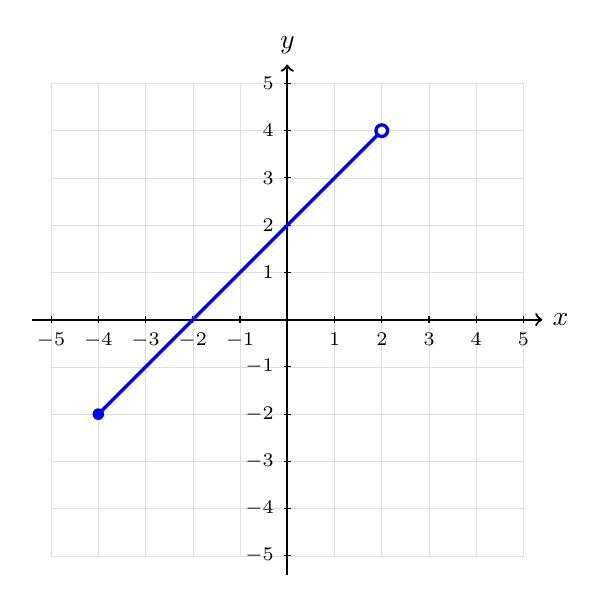
\begin{tikzpicture}[scale=0.6]
  \gridaxes{5}
  \draw[very thick,blue] (-4,-2)--(2,4);
  \fill[blue](-4,-2) circle(3.5pt);
  \fill[white](2,4) circle(3.5pt); \draw[very thick,blue](2,4) circle(3.5pt);
\end{tikzpicture}
\end{center}

Domain: $\underline{\hspace{4.5cm}}$ \hfill Range: $\underline{\hspace{4.5cm}}$

% ===========================================================================
\newpage
\section*{Limits --- Reading, Tables \& Concepts}

\textbf{20.}\quad[16 pts]\quad Use the graph of $H$ below (the dashed line is a vertical asymptote). Open circles
are missing points; filled circles are actual values.

\begin{center}
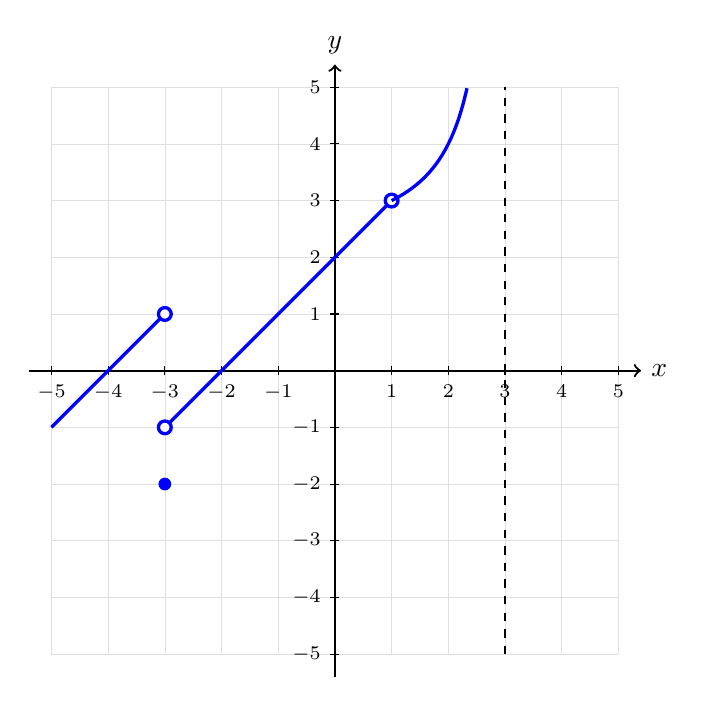
\begin{tikzpicture}[scale=0.72]
  \gridaxes{5}
  \draw[dashed] (3,-5)--(3,5);
  \draw[very thick,blue] (-5,-1)--(-3,1);
  \fill[white](-3,1) circle(3.2pt); \draw[very thick,blue](-3,1) circle(3.2pt);
  \fill[blue](-3,-2) circle(3.2pt);
  \draw[very thick,blue] (-3,-1)--(1,3);
  \fill[white](-3,-1) circle(3.2pt); \draw[very thick,blue](-3,-1) circle(3.2pt);
  \fill[white](1,3) circle(3.2pt); \draw[very thick,blue](1,3) circle(3.2pt);
  \draw[very thick,blue,domain=1:2.33,samples=100] plot(\x,{3+(\x-1)/(3-\x)});
\end{tikzpicture}
\end{center}

\textbf{(a)} $\displaystyle\lim_{x \to -3^-} H(x) = \underline{\hspace{1.5cm}}$\quad
\textbf{(b)} $\displaystyle\lim_{x \to -3^+} H(x) = \underline{\hspace{1.5cm}}$\quad
\textbf{(c)} $\displaystyle\lim_{x \to -3} H(x) = \underline{\hspace{1.5cm}}$

\medskip
\textbf{(d)} $H(-3) = \underline{\hspace{1.5cm}}$\quad
\textbf{(e)} $\displaystyle\lim_{x \to 1} H(x) = \underline{\hspace{1.5cm}}$\quad
\textbf{(f)} Is $H(1)$ defined? $\underline{\hspace{2cm}}$

\medskip
\textbf{(g)} $\displaystyle\lim_{x \to 3^-} H(x) = \underline{\hspace{1.5cm}}$

\newpage
\textbf{21.}\quad[6 pts]\quad The table shows values of $f(x) = \dfrac{x^2 - 4}{\,x - 2\,}$ near $x = 2$.

\medskip
\renewcommand{\arraystretch}{1.4}
\begin{tabular}{|C{1.5cm}|C{1.4cm}|C{1.4cm}|C{1.6cm}|C{1.6cm}|C{1.4cm}|C{1.4cm}|}
\hline
$x$ & $1.9$ & $1.99$ & $1.999$ & $2.001$ & $2.01$ & $2.1$ \\
\hline
$f(x)$ & $3.9$ & $3.99$ & $3.999$ & $4.001$ & $4.01$ & $4.1$ \\
\hline
\end{tabular}
\renewcommand{\arraystretch}{1}

\medskip
\textbf{(a)}\quad $\displaystyle\lim_{x \to 2} f(x) = \underline{\hspace{2.5cm}}$ 

\textbf{(b)}\quad Is $f(2)$ defined? Why or why not?
\wl

\bigskip
\textbf{22.}\quad[8 pts]\quad In your own words:

\medskip
\textbf{(a)}\quad Explain the difference between saying ``$\displaystyle\lim_{x \to a} f(x)$ does not exist'' and
saying ``$f(a)$ is undefined.''
\wls{2}

\textbf{(b)}\quad Describe or sketch a function for which the limit at a point \emph{exists} even though the
function is \emph{undefined} there.
\begin{center}
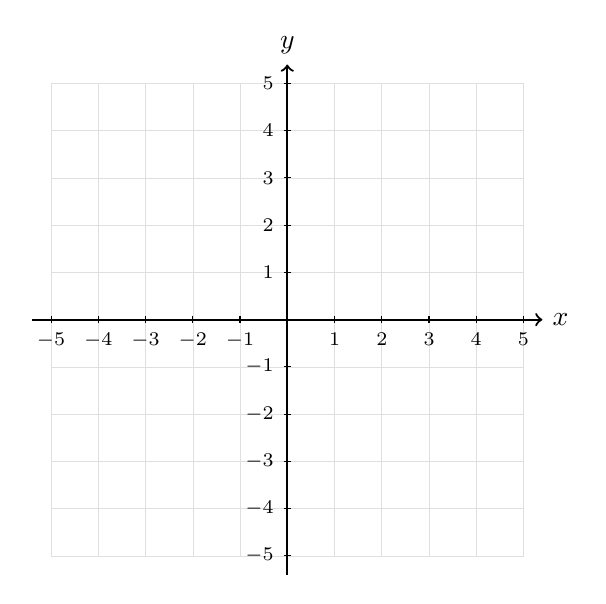
\begin{tikzpicture}[scale=0.6]
  \gridaxes{5}
\end{tikzpicture}
\end{center}


% ===========================================================================
\newpage
\section*{Finding Limits with Algebra}

\textbf{23.}\quad[22 pts]\quad Evaluate each limit. Show your steps.

\medskip
\textbf{(a)}\quad[3]\quad $\displaystyle\lim_{x \to 2} \big(x^2 - 3x + 1\big)$
\vspace{8em}

\textbf{(b)}\quad[4]\quad $\displaystyle\lim_{x \to 4} \frac{x^2 - 16}{\,x - 4\,}$
\vspace{15em}

\textbf{(c)}\quad[4]\quad $\displaystyle\lim_{x \to -1} \frac{x^2 - 1}{\,x^2 + 3x + 2\,}$

\newpage
\textbf{(d)}\quad[4]\quad For $\;f(x) = \begin{cases} x + 4 & x < 2 \\ x^2 - 1 & x \ge 2 \end{cases}$,\;
find $\displaystyle\lim_{x \to 2^-} f(x)$, $\displaystyle\lim_{x \to 2^+} f(x)$, and $\displaystyle\lim_{x \to 2}
f(x)$.
\vspace{18em}

\textbf{(e)}\quad[4]\quad $\displaystyle\lim_{x \to 2^+} \frac{1}{\,x - 2\,}$ \;and\;
$\displaystyle\lim_{x \to 2^-} \frac{1}{\,x - 2\,}$.\; Does $\displaystyle\lim_{x \to 2} \frac{1}{\,x - 2\,}$ exist?

% ===========================================================================
\newpage
\section*{Limits at Infinity (End Behavior)}

\textbf{24.}\quad[12 pts]\quad Find each limit using the dominant-term shortcut. State whether the answer is
a number, $0$, $+\infty$, or $-\infty$.

\medskip
\textbf{(a)}\quad $\displaystyle\lim_{x \to \infty} \frac{5x^3 - 2x}{\,2x^3 + 7\,}$
\vspace{6em}

\textbf{(b)}\quad $\displaystyle\lim_{x \to \infty} \frac{3x + 1}{\,x^2 - 4\,}$
\vspace{6em}

\textbf{(c)}\quad $\displaystyle\lim_{x \to \infty} \frac{x^2 + 5}{\,4x + 1\,}$
\vspace{6em}

\textbf{(d)}\quad $\displaystyle\lim_{x \to \infty} \frac{6x^2 - x}{\,2x^2 + 3x - 5\,}$
\vspace{6em}

\newpage
\textbf{25.}\quad[14 pts]\quad Now do it rigorously: divide the top and bottom by the highest power of
$x$, and use the fact that $\displaystyle\lim_{x\to\infty}\tfrac{1}{x^n} = 0$. For each step state which limit law you are using.

\medskip
$\displaystyle\lim_{x \to \infty} \frac{2x^2 - x}{\,5x^2 + 4\,}$

\newpage
\textbf{26.}\quad What was the hardest part of our math classes? Do you believe one day in the future you'll be able to conquer it?

\end{document}
